\chapter{Implementierung der Client-Schnittstelle}
\label{cha:impl_api}

Die Client-Schnittstelle dient der Kommunikation zwischen den Clients (z.B. Smartglass) und dem \acs{SMAR}-Server, um Zugriff auf die Daten aus der Datenbank zu erhalten und diese zu manipulieren.\\

Für diese Client-Schnittstelle fiel die Wahl auf eine \acs{REST} \acs{API}. Dabei handelt es sich um einen Webservice, der Ressourcen über fest definierte Routen (virtuelle Dateipfade auf dem Server) bereitstellt. Diese Routen können über die Standard-\acs{HTTP}-Befehle wie z.B. \emph{GET} oder \emph{POST} angesprochen werden und sind somit technologisch sehr flexibel -- \acs{HTTP}-Anfragen können von fast allen Programmiersprachen und -umgebungen versendet und empfangen werden.\\

Die \acs{API} wird nicht nur von externen Clients verwendet. Auch die Webadministration greift zum Teil auf \acs{REST} Services zu, teilweise wurden Services explizit für die Webadministration implementiert. Anwendungsbeispiele sind asynchrone \acs{AJAX}-Requests, die Funktionen wie Autovervollständigung in Formularfeldern bedienen und über einen Service optimal mit Daten versorgt werden können.

\section{Technologische Grundlagen}
Wie die Webadministration wurde die \acs{REST} \acs{API} über die Scriptsprache \acs{PHP} umgesetzt. Um den Arbeitsaufwand möglichst gering zu halten und gleichzeitig eine stabile API bereitstellen zu können, wurde das \emph{Slim Framework}(\url{http://www.slimframework.com/}) verwendet. Dabei handelt es sich um ein leichtgewichtiges Framework, mit dem Routen für die gängigen \acs{HTTP}-Befehle in \acs{PHP} programmiert werden. Das Format für den Datenaustausch ist dabei nicht vorgegeben, die Kommunikation wird im Rahmen von Webapplikationen jedoch in der Regel auf JSON basiert.\\

Der Ablauf eines Kommunikationszyklusses gestaltet sich analog zu einem regulären \acs{HTTP}-Request. Der Client sendet eine Anfrage an den entsprechenden \acs{URL} des \acs{REST} Service, den der Client ansprechen möchte. Abhängig vom Service muss der Request \emph{GET} oder \emph{POST} als Methode verwenden, sowie u.U. notwendige Parameter für die Anfrage enthalten. Der Webserver empfängt die Anfrage und leitet sie aufgrund der Konfiguration des Slim Frameworks an die \acs{API} weiter. Diese ordnet die Route einer Programmroutine zu, welche entsprechend der Anfrage Daten zurückliefert. Dazu werden vom REST Service eventuell Datenbankabfragen durchgeführt.

\section{PHP JWT}
\label{cha:jwt}
\sloppy

Bei der in diesem Projekt genutzten Bibliotek \glqq PHP JWT\grqq\ handelt es sich um eine objektorientierte \ac{PHP}-Klasse von \mbox{\url{firebase.com}} zur Generierung von \acl{JWT}.
\fussy
\begin{figure}[H]
	\centering
	{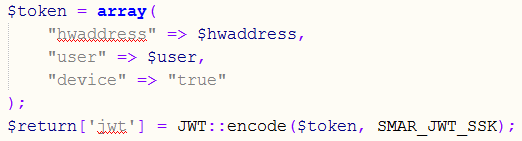
\includegraphics[scale=1.0]{Bilder/jwt_encode.png}}
	\caption{Generierung eines \acs{JWT}}
	\label{fig:jwt_encode}
\end{figure}

Abbildung \ref{fig:jwt_encode} zeigt die Generierung eines \ac{JWT}. \$token beschreibt dabei das \ac{JSON}-Objekt und enthält den Inhalt. SMAR\_JWT\_SSK ist eine in der Konfigurationsdatei festgelegte Konstante und beschreibt den Secret Server Key (geheimer Schlüssel), der nur dem Server bekannt ist, anhand dessen der Inhalt signiert wird. Dadurch wird sichergestellt, dass der \ac{JWT} bei einer weiteren Anfrage an den Server nicht durch den Client manipuliert wurde.\\

Die Dekodierung eines solchen \acl{JWT} wird in Abbildung \ref{fig:jwt_decode} beschrieben. Dabei muss SMAR\_JWT\_SSK (Secret Server Key) identisch zu dem Schlüssel sein, der zur Generierung des \ac{JWT} benutzt wurde. Sind die Schlüssel nicht identisch, wird der Token nicht dekodiert und die Funktion liefert ein leeres Ergebnis zurück.

\begin{figure}[H]
	\centering
	{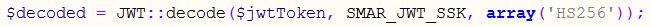
\includegraphics[scale=1.0]{Bilder/jwt_decode.png}}
	\caption{Dekodieren eines \acs{JWT}}
	\label{fig:jwt_decode}
\end{figure}

Ein \ac{JSON} Web Token setzt sich aus folgenden drei Abschnitten zusammen:\footnote{\citep[S. 289f.]{book_jwt}}
\begin{enumerate}
	\item JSON-Objekt, welches den \acs{JWT}-Header repräsentiert
	\item JSON-Objekt bestehend aus verschiedenen Name/Wert-Paaren (Claims-Set), welche die Daten des Benutzers enthält, in diesem Projekt \zB:
	\begin{itemize}
		\item die \acs{MAC}-Adresse des Gerätes und
		\item den Benutzernamen des angemeldeten Benutzers
	\end{itemize}
	\item die Signatur
\end{enumerate}
Alle drei Abschnitte sind jeweils mit BASE64-codiert und werden durch einen Punkt (.) voneinander getrennt.\\

Der \acs{JWT}-Header besteht ebenfalls aus zwei Name/Wert-Paaren und sieht in diesem Projekt wie folgt aus:
\begin{figure}[H]
	\centering
	{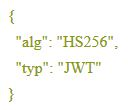
\includegraphics[scale=1.0]{Bilder/jwt_header.jpg}}
	\caption{\acs{JWT}-Header}
	\label{fig:jwt_header}
\end{figure}
Der Header beschreibt den Typ (JWT) und den verwendeten Algorithmus \shorthandoff{"} ("alg":"HS256") \shorthandon{"} zur Signierung. In \ac{SMAR} wurde der HS256-Algorithmus zur Signierung des Claims-Set verwendet. Das Claims-Set wurde somit mit einem privaten Schlüssel und SHA-256 zu einem Hash-Wert errechnet (dies ist der dritte Teil des \acs{JWT}). Die Signierung kann aufgrund des symmetrischen Signierungsalgorithmus außerdem nur mit dem selben privaten Schlüssel überprüft werden.\\
Ein \acl{JWT} stellt somit die Identität der Nachricht \bzw des \ac{JSON}-Objekt sicher und verhindert die unbemerkte Manipulation.\\

Durch den Einsatz von PHP JWT wird in \ac{SMAR} die korrekt authentifizierte Kommunikation mit der REST API - sowohl von der App, als auch von der Web Administration - sichergestellt.
Mit der Anmeldung an der Brille \bzw an der Weboberfläche wird eine Authentifizierungsanfrage an den Server (Web Administration) oder an die REST Api (\acs{VR}-Gerät) gestellt, ist die \acl{AuthN} erfolgreich, so wird ein gültiger \ac{JWT} mit Hilfe der PHP JWT-Klasse generiert. Dieser wird an die PHP-Session in der Web Administration oder an das \acs{VR}-Gerät zurückgegeben. Bei einer Anfrage an die REST Api muss dieser \acs{JWT} mitgegeben werden. Die REST Api dekodiert bei einer Anfrage zunächst den Token mit PHP JWT. Ist die Signatur gültig, wird ein JSON-Objekt zurückgegeben, ansonsten gibt es nur eine leere Antwort. Anschließend werden die Daten des JSON-Objekts mit der Datenbank verglichen, dies stellt sicher, dass die Berechtigung zur Ausführung noch vorhanden ist. Ist auch dies Erfolgreich wird die Anfrage ausgeführt. Bei einem Fehlerfall wird die Anfrage mit einer Fehlermeldung revidiert.

\section{REST Services}
Die Routen der \acs{REST} Services starten alle im Unterordner \emph{/api} des Web-Interfaces. Routen müssen nicht nur statisch sein, sondern können auch Parameter enthalten -- entsprechend der Philosophie von \acs{REST} Services, bereits über den \acs{URL} die angesprochene(n) Ressource(n) zu definieren. Die folgende Liste soll alle relevanten Services kurz vorstellen.

\begin{description}
  \item[/authenticate] \hfill \\
    Dieser Service dient zur initialen Anmeldung an der \acs{API} und liefert einen Token (\acs{JWT}) zurück, der bei den folgenden Requests zur Authentifizierung verwendet wird.
  \item[/sections/:shelfid] \hfill \\
    Gibt den kompletten Datenbankeintrag einer Section (Regalplatz) mit der übergebenen ID (\emph{shelfid}) zurück.
  \item[/barcode/:barcode] \hfill \\
    Sucht in der Datenbank nach dem Objekt mit dem übergebenen Barcode (in Tabellen \textit{\textbf{product}}, \textit{\textbf{product\_unit}}, \textit{\textbf{shelf}}) und gibt den kompletten Datensatz bei Fund zurück.
  \item[/search/:table/:search(/:limit)] \hfill \\
    Dieser Service bedient Autovervollständigungsfelder in Formularen der Webadministration. Zu einer gegebenen Tabelle und einem Suchbegriff gibt der Dienst passende Datensätze (optional in limitierter Menge) zurück.
  \item[/designer/update/:shelfid] \hfill \\
    Der Speicherbutton des Shelf Designers in der Webadministration sendet die Anordnung der Sections an diesen Service, welcher die Positionen und Größen der Sections in der Datenbank updatet und auch die Grafik für das Regal neu generiert.
\end{description}
